\documentclass{article}

\usepackage{graphicx}
\usepackage{tikz}
\usepackage{tikzsymbols}
\usetikzlibrary{calc,patterns,shapes.geometric}
\pagestyle{empty}
\usepackage[margin=0pt]{geometry}
\geometry{papersize={14in,12in}}

\def\centerarc[#1](#2)(#3:#4:#5){\draw[#1] ($(#2)+({#5*cos(#3)},{#5*sin(#3)})$) arc (#3:#4:#5);}

\begin{document}
	\begin{figure}
		\centering
		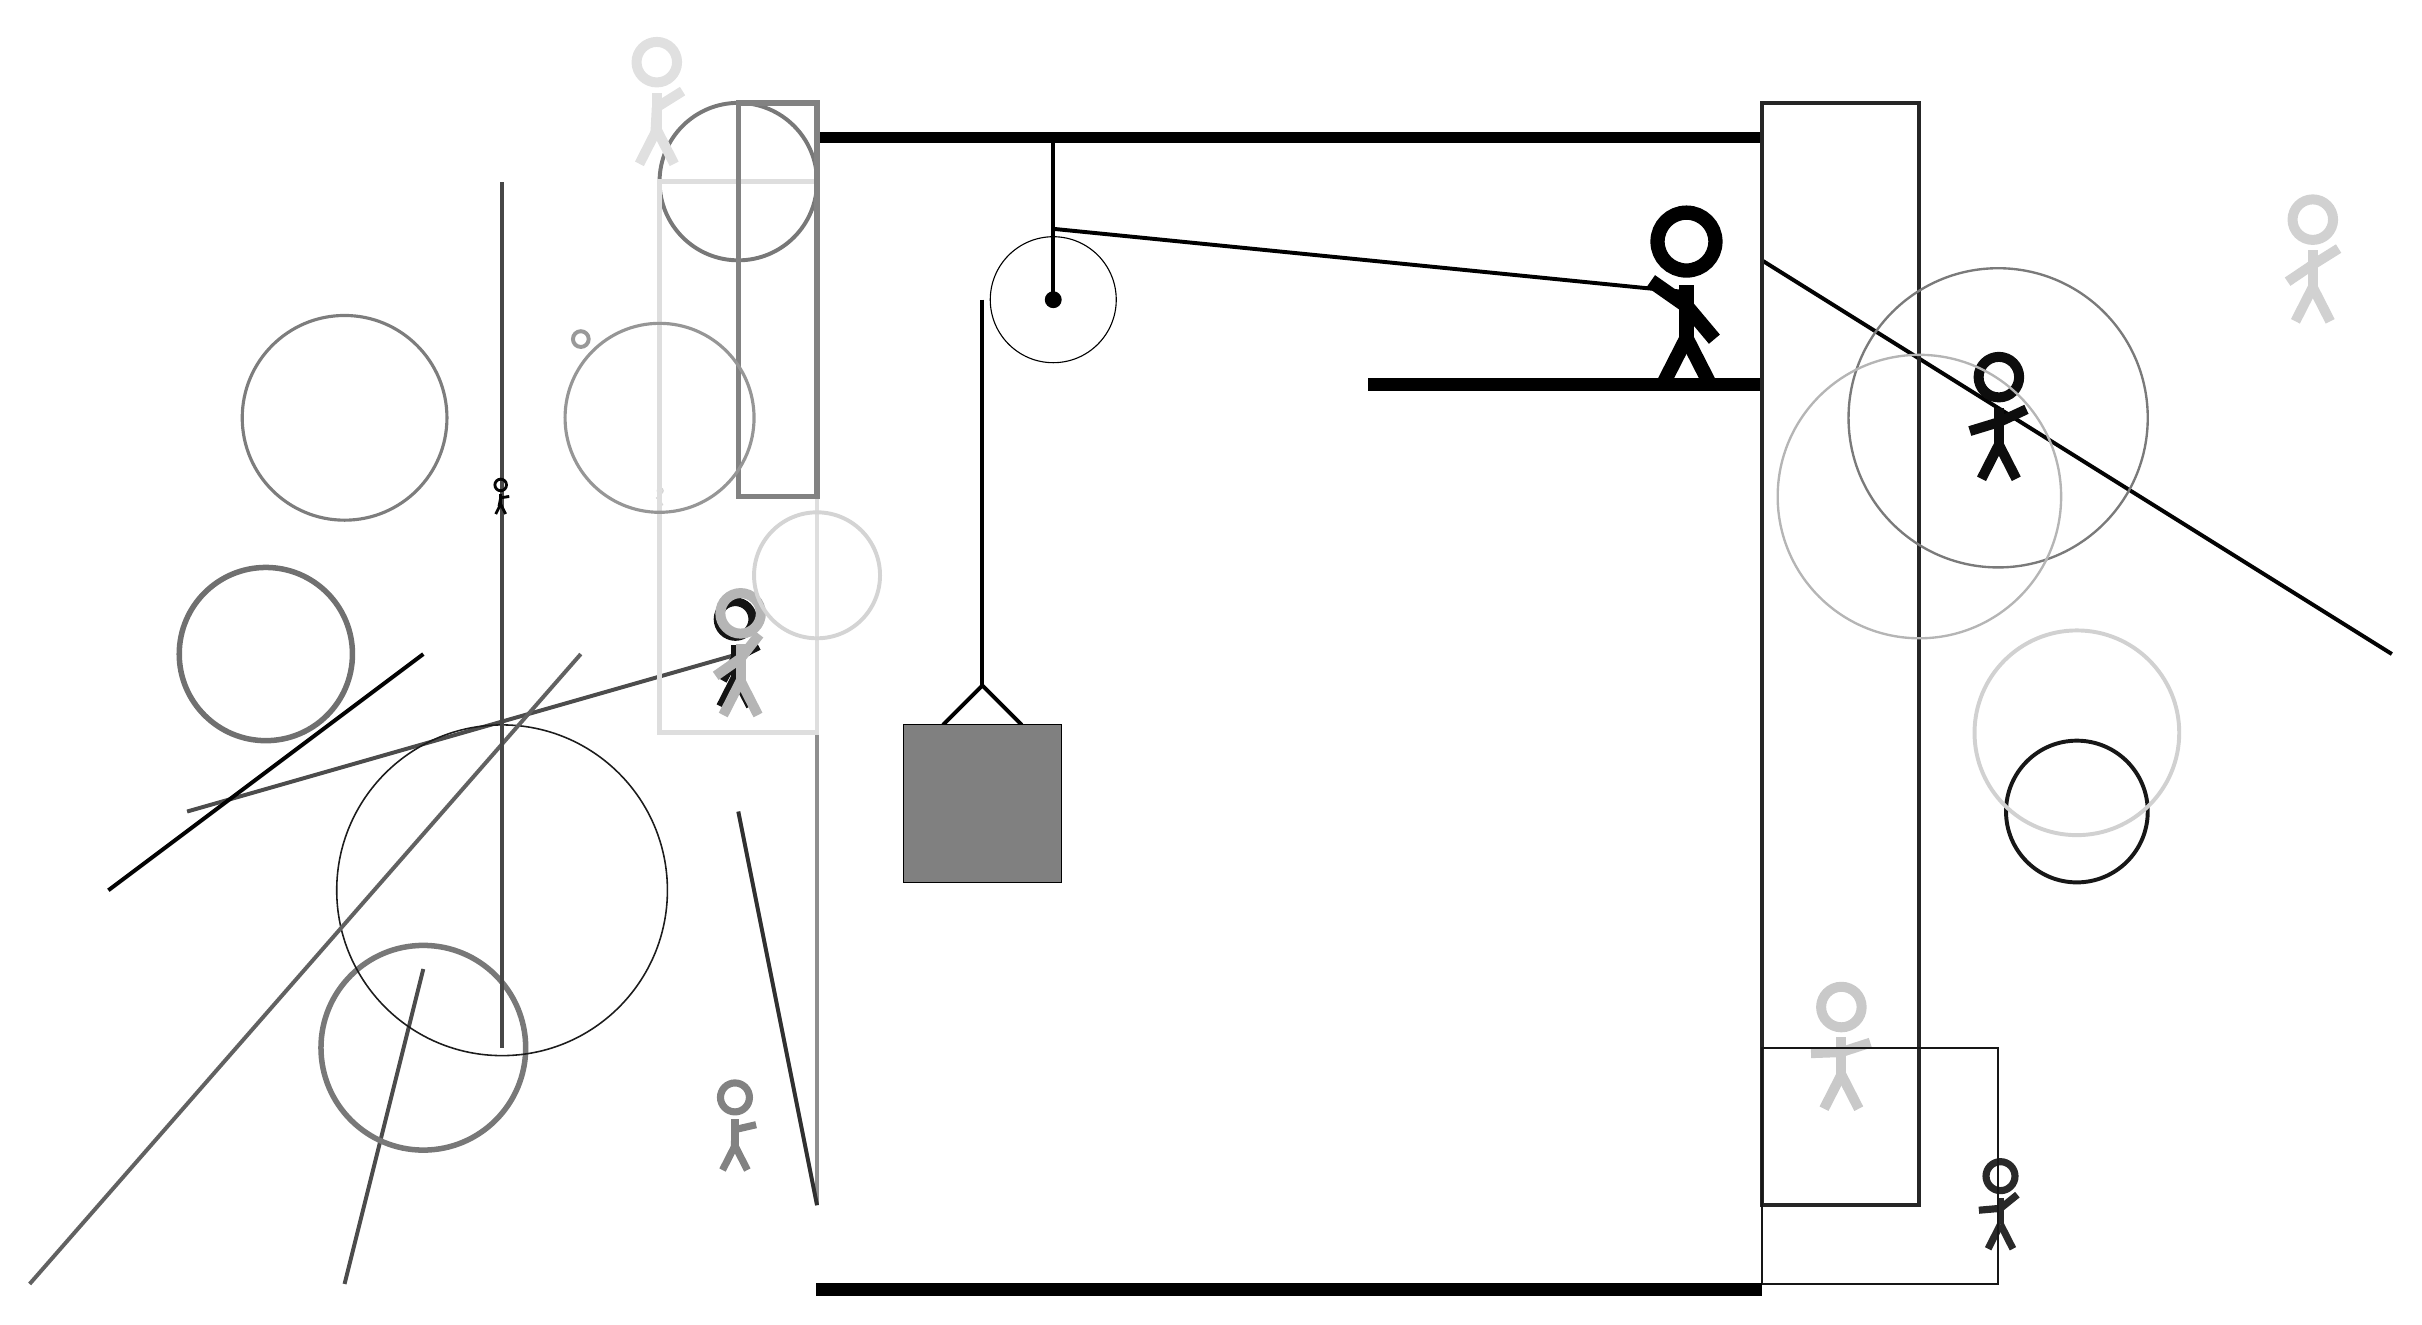
\begin{tikzpicture}
			%%%%% START %%%%%
			
			\draw[fill=black] (-2, 11.5) rectangle (10, 11.625);
			
			\draw (1, 9.5) circle (0.8);
			\draw[fill=black] (1, 9.5) circle (0.1);
			\draw[line width=0.5mm] (1, 11.5) -- (1, 9.5);
			
			\draw[line width=0.5mm](-0.4, 4.1) --  (0.1, 4.6) -- (0.6, 4.1);
			\draw[fill=black!50] (-0.9, 4.1) rectangle (1.1, 2.1);
			
			\draw[line width=0.5mm](0.1, 9.5) -- (0.1, 4.6);
			\centerarc[line width=0.5mm](1, 9.5)(90:180:0.9)
			\draw[line width=0.5mm](1, 10.4) -- (9, 9.6);
			
			\node at (9, 9.5) {\Strichmaxerl[10][-35][-50]};
			\draw[fill=black] (5, 8.5) rectangle (10, 8.35);
			
			\node[line width=0.5mm, color=black!16] at (-4, 7) {\Strichmaxerl[1][12][80]};
			
			\draw [line width=0.5mm, color=black!91](14, 3) circle (0.9);
			\draw[line width=0.5mm, color=black!99](10, 10) -- (18, 5);
			\draw [line width=0.4mm, color=black!51](-8, 8) circle (1.3);
			
			\draw [line width=0.5mm, color=black!53](-3, 11) circle (1.0);
			\draw[line width=0.5mm, color=black!70](-3, 5) -- (-10, 3);
			
			\node[line width=0.6mm, color=black!21] at (11, 0) {\Strichmaxerl[7][2][18]};
			\node[line width=0.3mm, color=black!92] at (-3, 5) {\Strichmaxerl[6][61][27]};
			\draw[line width=0.5mm, color=black!70](-7, 1) -- (-8, -3);
			\node[line width=0.3mm, color=black!29] at (-3, 5) {\Strichmaxerl[7][35][52]};
			\draw [line width=0.7mm, color=black!53](-7, 0) circle (1.3);
			
			\draw[line width=0.5mm, color=black!44] (-2, 8) rectangle (-2, -2);
			\node[line width=0.6mm, color=black!18] at (17, 10) {\Strichmaxerl[7][34][32]};
			
			\draw[line width=0.6mm, color=black!13] (-4, 4) rectangle (-2, 11);
			\draw[line width=0.5mm, color=black!85] (12, 12) rectangle (10, -2);
			\draw[line width=0.5mm, color=black!81](-2, -2) -- (-3, 3);
			
			\draw [line width=0.3mm, color=black!52](13, 8) circle (1.9);
			\node[line width=0.7mm, color=black!12] at (-4, 12) {\Strichmaxerl[7][87][32]};
			\draw[line width=0.7mm, color=black!49] (-3, 12) rectangle (-2, 7);
			\node[line width=0.7mm, color=black!84] at (13, -2) {\Strichmaxerl[5][5][39]};
			\draw [line width=0.4mm, color=black!41](-4, 8) circle (1.2);
			\draw [line width=0.2mm, color=black!89](-6, 2) circle (2.1);
			
			\draw[line width=0.5mm, color=black!99](-7, 5) -- (-11, 2);
			\draw[line width=0.5mm, color=black!62](-5, 5) -- (-12, -3);
			\node[line width=0.7mm, color=black!49] at (-3, -1) {\Strichmaxerl[5][88][13]};
			
			\draw [line width=0.5mm, color=black!18](14, 4) circle (1.3);
			
			\draw [line width=0.5mm, color=black!40](-5, 9) circle (0.1);
			\node[line width=0.3mm, color=black!95] at (13, 8) {\Strichmaxerl[7][17][25]};
			
			\draw [line width=0.3mm, color=black!29](12, 7) circle (1.8);
			\draw [line width=0.7mm, color=black!56](-9, 5) circle (1.1);
			\draw[line width=0.3mm, color=black!91] (10, -3) rectangle (13, 0);
			
			\draw[line width=0.5mm, color=black!72](-6, 0) -- (-6, 11);
			\draw [line width=0.5mm, color=black!17](-2, 6) circle (0.8);
			\node[line width=0.3mm, color=black!98] at (-6, 7) {\Strichmaxerl[2][79][9]};
			
			\draw[fill=black] (-2, -3) rectangle (10, -3.15);
			
			%%%%% END %%%%%
		\end{tikzpicture}
	\end{figure}	
\end{document}